\SourceLeaf{238}%
der parallelen Fortbewegung von $GK$ nach $AB$ einen \textls{letzten} Punkt $N$ in $ED$
\begin{center}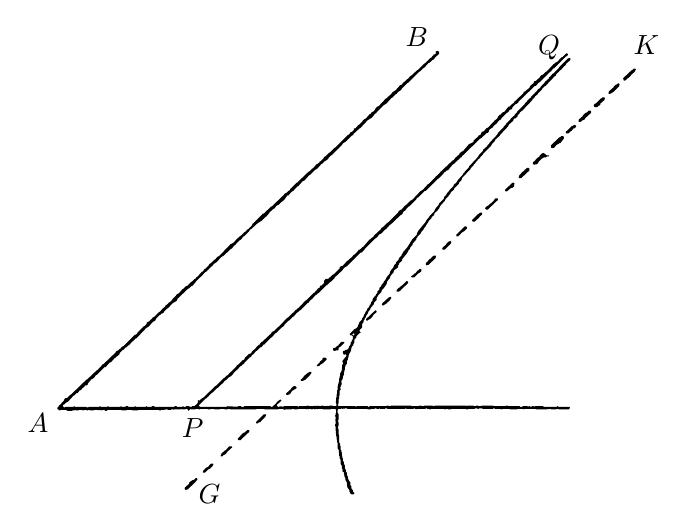
\begin{tikzpicture}[x=0.00643910cm,y=-0.00643910cm]
\fill[even odd rule] (356,910) -- (355,909) -- (353,909) -- (350,912) -- (346,913) -- (344,915) -- (343,915) -- (340,918) -- (340,920) -- (332,927) -- (331,930) -- (333,932) -- (337,931) -- (353,916) -- (353,915) -- (356,912) -- cycle
(388,881) -- (387,880) -- (384,880) -- (382,881) -- (377,887) -- (374,888) -- (368,894) -- (367,897) -- (368,898) -- (371,898) -- (377,892) -- (381,890) -- (386,885) -- cycle
(425,847) -- (424,846) -- (419,846) -- (412,854) -- (411,854) -- (404,860) -- (402,865) -- (403,866) -- (405,866) -- (408,863) -- (411,862) -- (414,859) -- (414,858) -- (425,848) -- cycle
(459,815) -- (458,814) -- (455,814) -- (449,819) -- (446,820) -- (436,831) -- (436,833) -- (437,834) -- (442,834) -- (443,832) -- (458,818) -- cycle
(492,784) -- (491,783) -- (487,783) -- (472,798) -- (472,800) -- (473,801) -- (475,801) -- (477,799) -- (481,798) -- (482,796) -- (490,788) -- cycle
(552,730) -- (549,727) -- (545,728) -- (541,732) -- (541,733) -- (531,742) -- (531,743) -- (533,745) -- (539,743) -- (542,738) -- (544,736) -- (551,732) -- cycle
(581,700) -- (580,699) -- (578,699) -- (573,702) -- (566,708) -- (566,709) -- (560,715) -- (560,716) -- (561,717) -- (564,717) -- (570,714) -- (579,705) -- (579,704) -- (581,702) -- cycle
(611,673) -- (608,671) -- (605,671) -- (603,673) -- (603,675) -- (598,679) -- (598,680) -- (592,686) -- (592,687) -- (593,688) -- (596,688) -- (600,684) -- (604,682) -- (611,675) -- cycle
(646,641) -- (645,640) -- (640,640) -- (633,648) -- (632,648) -- (628,652) -- (625,652) -- (624,653) -- (624,656) -- (626,658) -- (628,658) -- (629,657) -- (633,657) -- (635,655) -- (635,652) -- (637,650) -- (638,650) -- (646,642) -- cycle
(710,580) -- (708,578) -- (707,578) -- (689,595) -- (689,597) -- (690,598) -- (692,598) -- (694,596) -- (697,595) -- (701,591) -- (704,586) -- (710,581) -- cycle
(739,553) -- (737,551) -- (733,553) -- (721,564) -- (720,567) -- (721,568) -- (724,568) -- (726,566) -- (727,566) -- (736,558) -- cycle
(772,522) -- (770,520) -- (769,520) -- (760,529) -- (759,529) -- (755,533) -- (754,533) -- (749,538) -- (749,540) -- (750,541) -- (754,541) -- (756,539) -- (757,539) -- (758,537) -- (772,524) -- cycle
(798,497) -- (797,496) -- (795,496) -- (792,499) -- (791,499) -- (786,505) -- (785,505) -- (781,509) -- (780,509) -- (778,511) -- (778,512) -- (779,513) -- (784,513) -- (792,505) -- (797,502) -- (798,500) -- cycle
(827,471) -- (826,470) -- (823,470) -- (821,471) -- (815,477) -- (814,477) -- (809,483) -- (807,484) -- (807,488) -- (808,489) -- (812,488) -- (826,475) -- cycle
(857,443) -- (855,441) -- (851,443) -- (847,447) -- (847,448) -- (840,454) -- (839,457) -- (840,458) -- (844,458) -- (856,446) -- cycle
(888,414) -- (886,412) -- (884,412) -- (869,427) -- (867,428) -- (867,431) -- (868,432) -- (870,432) -- (872,430) -- (873,430) -- (877,425) -- (882,422) -- (888,416) -- cycle
(918,386) -- (917,385) -- (914,385) -- (911,388) -- (910,388) -- (898,400) -- (898,401) -- (900,403) -- (903,403) -- (908,398) -- (909,398) -- (915,391) -- (917,390) -- cycle
(949,358) -- (948,357) -- (944,357) -- (942,359) -- (942,360) -- (935,367) -- (934,367) -- (929,372) -- (928,372) -- (924,376) -- (924,377) -- (926,379) -- (929,379) -- (949,360) -- cycle
(982,328) -- (980,326) -- (978,326) -- (963,340) -- (963,342) -- (964,343) -- (967,343) -- (974,337) -- (978,336) -- (981,333) -- (981,330) -- cycle
(1011,298) -- (1010,297) -- (1006,297) -- (1003,300) -- (1002,300) -- (1001,302) -- (999,304) -- (998,304) -- (991,312) -- (990,316) -- (991,317) -- (995,317) -- (1011,302) -- cycle
(1050,273) -- (1049,272) -- (1045,272) -- (1040,268) -- (1037,268) -- (1035,269) -- (1031,273) -- (1031,274) -- (1029,276) -- (1028,276) -- (1023,281) -- (1023,282) -- (1018,286) -- (1018,289) -- (1020,291) -- (1022,290) -- (1025,290) -- (1029,287) -- (1029,285) -- (1035,279) -- (1040,276) -- (1044,276) -- (1046,274) -- (1050,274) -- cycle
(1079,236) -- (1077,234) -- (1074,234) -- (1072,236) -- (1071,236) -- (1054,252) -- (1054,257) -- (1055,258) -- (1060,257) -- (1065,251) -- (1068,250) -- (1070,248) -- (1072,248) -- (1079,239) -- cycle
(1103,214) -- (1101,212) -- (1099,212) -- (1097,214) -- (1095,214) -- (1085,224) -- (1083,225) -- (1083,228) -- (1084,229) -- (1087,229) -- (1089,228) -- (1093,224) -- (1094,224) -- (1098,219) -- (1100,219) -- (1103,216) -- cycle
(1133,186) -- (1131,184) -- (1128,184) -- (1125,187) -- (1121,189) -- (1116,194) -- (1116,195) -- (1108,202) -- (1108,205) -- (1109,206) -- (1112,206) -- (1116,203) -- (1119,202) -- (1121,200) -- (1121,199) -- (1133,188) -- cycle
(1160,159) -- (1159,158) -- (1155,158) -- (1153,160) -- (1152,160) -- (1143,169) -- (1138,172) -- (1139,176) -- (1140,177) -- (1145,177) -- (1148,174) -- (1149,174) -- (1151,172) -- (1151,170) -- (1159,163) -- cycle
(1189,132) -- (1187,130) -- (1186,130) -- (1184,132) -- (1180,134) -- (1177,137) -- (1177,138) -- (1168,146) -- (1167,150) -- (1168,151) -- (1170,151) -- (1177,147) -- (1188,136) -- cycle
(1220,101) -- (1217,101) -- (1214,104) -- (1213,104) -- (1196,120) -- (1197,124) -- (1198,125) -- (1201,124) -- (1205,120) -- (1206,120) -- (1211,115) -- (1211,114) -- (1218,108) -- (1221,103) -- cycle
(1087,73) -- (1085,71) -- (1084,71) -- (1077,78) -- (1074,79) -- (1066,88) -- (1063,89) -- (1060,92) -- (1059,92) -- (1045,107) -- (1044,107) -- (1038,113) -- (1035,114) -- (1032,117) -- (1032,118) -- (1023,126) -- (1021,126) -- (1020,127) -- (1020,129) -- (1012,136) -- (1012,138) -- (1008,142) -- (1007,142) -- (1003,146) -- (1002,146) -- (999,149) -- (999,150) -- (981,167) -- (981,168) -- (979,170) -- (978,170) -- (972,176) -- (970,176) -- (962,186) -- (959,187) -- (954,192) -- (953,192) -- (949,196) -- (948,199) -- (945,202) -- (944,202) -- (930,217) -- (926,219) -- (921,225) -- (919,225) -- (916,228) -- (916,230) -- (914,232) -- (911,233) -- (910,235) -- (901,243) -- (901,245) -- (899,247) -- (892,250) -- (880,264) -- (877,265) -- (873,269) -- (873,270) -- (864,278) -- (864,279) -- (861,282) -- (860,282) -- (854,288) -- (853,288) -- (848,294) -- (847,294) -- (837,304) -- (836,304) -- (835,306) -- (828,313) -- (827,313) -- (826,315) -- (812,329) -- (811,329) -- (801,340) -- (796,343) -- (781,359) -- (776,362) -- (767,371) -- (766,371) -- (759,379) -- (756,380) -- (752,384) -- (752,385) -- (732,405) -- (731,405) -- (722,414) -- (721,414) -- (718,417) -- (718,418) -- (704,431) -- (704,432) -- (702,434) -- (701,434) -- (697,438) -- (696,438) -- (683,453) -- (682,453) -- (678,457) -- (673,460) -- (672,462) -- (666,468) -- (665,468) -- (659,475) -- (658,475) -- (653,480) -- (652,480) -- (643,490) -- (639,491) -- (637,493) -- (637,495) -- (625,507) -- (624,507) -- (614,516) -- (609,516) -- (606,520) -- (606,524) -- (601,529) -- (599,529) -- (598,530) -- (598,532) -- (596,534) -- (595,534) -- (587,543) -- (586,543) -- (571,558) -- (570,558) -- (556,573) -- (555,573) -- (551,577) -- (550,577) -- (545,583) -- (544,583) -- (535,592) -- (534,592) -- (517,610) -- (516,610) -- (507,619) -- (504,620) -- (502,622) -- (502,623) -- (499,626) -- (498,626) -- (497,628) -- (484,640) -- (483,640) -- (480,643) -- (480,644) -- (478,646) -- (477,646) -- (472,651) -- (472,652) -- (463,660) -- (463,661) -- (461,663) -- (458,664) -- (452,670) -- (451,670) -- (449,674) -- (447,676) -- (446,676) -- (436,686) -- (435,686) -- (433,688) -- (433,689) -- (422,700) -- (421,700) -- (416,706) -- (415,706) -- (410,711) -- (409,711) -- (393,727) -- (392,727) -- (367,751) -- (366,751) -- (360,756) -- (357,755) -- (357,760) -- (356,762) -- (350,767) -- (346,767) -- (345,768) -- (341,768) -- (340,767) -- (334,767) -- (333,768) -- (329,768) -- (328,767) -- (326,768) -- (316,768) -- (315,767) -- (312,767) -- (311,768) -- (272,768) -- (271,767) -- (267,767) -- (266,768) -- (257,768) -- (256,767) -- (254,768) -- (235,768) -- (234,767) -- (232,768) -- (220,768) -- (219,767) -- (215,767) -- (214,768) -- (207,768) -- (206,767) -- (204,768) -- (181,768) -- (180,767) -- (178,768) -- (166,768) -- (164,767) -- (163,768) -- (142,768) -- (141,769) -- (138,769) -- (137,768) -- (115,768) -- (113,767) -- (112,768) -- (96,768) -- (95,769) -- (93,769) -- (91,767) -- (91,765) -- (92,764) -- (93,764) -- (97,760) -- (101,758) -- (112,746) -- (113,746) -- (118,741) -- (120,741) -- (124,736) -- (127,735) -- (128,733) -- (131,730) -- (132,730) -- (135,726) -- (138,726) -- (140,724) -- (141,721) -- (147,714) -- (151,712) -- (154,709) -- (154,708) -- (157,705) -- (158,705) -- (173,690) -- (175,690) -- (183,681) -- (186,680) -- (193,672) -- (194,672) -- (198,668) -- (199,668) -- (203,664) -- (203,662) -- (209,656) -- (210,656) -- (215,651) -- (216,651) -- (220,647) -- (221,647) -- (228,639) -- (229,639) -- (235,633) -- (236,633) -- (255,613) -- (260,610) -- (268,601) -- (273,598) -- (275,594) -- (282,587) -- (283,587) -- (286,584) -- (288,584) -- (290,582) -- (290,581) -- (297,574) -- (298,574) -- (307,564) -- (314,560) -- (316,558) -- (317,555) -- (338,535) -- (339,535) -- (344,530) -- (346,530) -- (353,522) -- (353,521) -- (362,512) -- (363,512) -- (372,502) -- (373,502) -- (384,491) -- (385,491) -- (389,486) -- (394,483) -- (403,473) -- (408,470) -- (423,456) -- (424,456) -- (426,454) -- (426,453) -- (431,448) -- (432,448) -- (433,446) -- (440,439) -- (441,439) -- (445,435) -- (445,434) -- (447,432) -- (448,432) -- (459,421) -- (459,420) -- (462,417) -- (463,417) -- (475,406) -- (483,401) -- (491,393) -- (492,393) -- (498,386) -- (498,385) -- (507,377) -- (508,377) -- (513,371) -- (516,370) -- (523,363) -- (524,363) -- (530,357) -- (530,356) -- (534,351) -- (536,351) -- (542,344) -- (547,341) -- (548,339) -- (554,333) -- (555,333) -- (564,323) -- (567,322) -- (577,311) -- (578,311) -- (588,301) -- (593,298) -- (601,289) -- (602,289) -- (607,284) -- (612,281) -- (615,278) -- (615,277) -- (620,272) -- (621,272) -- (642,251) -- (642,250) -- (644,248) -- (649,245) -- (661,233) -- (663,233) -- (664,232) -- (664,230) -- (676,219) -- (677,219) -- (692,203) -- (700,198) -- (704,194) -- (704,193) -- (708,189) -- (709,189) -- (710,187) -- (724,173) -- (729,170) -- (739,159) -- (740,159) -- (748,151) -- (749,151) -- (752,147) -- (757,144) -- (759,142) -- (759,141) -- (771,129) -- (772,129) -- (794,107) -- (795,107) -- (802,100) -- (803,100) -- (812,90) -- (815,89) -- (820,84) -- (821,84) -- (825,80) -- (825,79) -- (832,73) -- (833,71) -- (833,68) -- (830,66) -- (827,67) -- (826,68) -- (827,71) -- (825,73) -- (823,73) -- (817,80) -- (816,80) -- (805,91) -- (804,91) -- (791,104) -- (790,104) -- (777,116) -- (776,116) -- (771,122) -- (770,122) -- (765,127) -- (764,127) -- (759,133) -- (756,134) -- (747,144) -- (742,147) -- (736,154) -- (735,154) -- (729,160) -- (728,160) -- (714,175) -- (711,176) -- (708,179) -- (706,183) -- (703,186) -- (700,187) -- (699,189) -- (697,191) -- (696,191) -- (689,199) -- (684,202) -- (682,204) -- (682,205) -- (675,212) -- (674,212) -- (668,219) -- (665,219) -- (665,222) -- (661,226) -- (658,227) -- (657,229) -- (654,232) -- (653,232) -- (628,257) -- (627,257) -- (617,267) -- (616,267) -- (609,274) -- (608,274) -- (605,277) -- (605,278) -- (599,284) -- (597,285) -- (597,286) -- (595,288) -- (592,289) -- (584,298) -- (583,298) -- (577,304) -- (576,304) -- (553,326) -- (552,326) -- (539,339) -- (539,340) -- (537,342) -- (536,342) -- (532,346) -- (528,348) -- (527,350) -- (503,373) -- (502,373) -- (487,387) -- (485,387) -- (484,389) -- (467,406) -- (465,407) -- (464,410) -- (456,418) -- (455,418) -- (451,423) -- (450,423) -- (442,431) -- (441,431) -- (437,435) -- (436,435) -- (427,445) -- (421,448) -- (399,471) -- (396,472) -- (391,478) -- (390,478) -- (383,485) -- (382,485) -- (379,488) -- (379,489) -- (372,496) -- (371,496) -- (369,498) -- (369,499) -- (366,502) -- (365,502) -- (356,512) -- (354,513) -- (354,514) -- (352,516) -- (351,516) -- (346,521) -- (345,521) -- (336,530) -- (334,530) -- (328,536) -- (327,536) -- (320,544) -- (315,547) -- (314,549) -- (307,556) -- (307,557) -- (302,562) -- (300,562) -- (299,564) -- (296,567) -- (295,567) -- (293,569) -- (293,570) -- (290,573) -- (289,573) -- (282,581) -- (281,581) -- (271,591) -- (268,592) -- (267,594) -- (265,596) -- (264,596) -- (261,600) -- (259,600) -- (256,603) -- (256,605) -- (252,609) -- (251,609) -- (238,622) -- (238,623) -- (236,625) -- (232,627) -- (211,648) -- (207,650) -- (204,654) -- (203,654) -- (200,657) -- (197,658) -- (195,660) -- (195,661) -- (171,684) -- (170,684) -- (159,696) -- (158,696) -- (139,714) -- (138,714) -- (107,744) -- (106,744) -- (99,751) -- (96,751) -- (94,753) -- (93,756) -- (88,761) -- (88,762) -- (83,766) -- (83,767) -- (80,770) -- (80,772) -- (84,775) -- (86,775) -- (87,774) -- (97,774) -- (100,776) -- (109,776) -- (110,775) -- (114,775) -- (115,774) -- (117,775) -- (122,775) -- (123,774) -- (129,774) -- (130,775) -- (133,775) -- (134,774) -- (137,774) -- (138,775) -- (140,775) -- (141,774) -- (143,774) -- (144,775) -- (152,775) -- (153,774) -- (169,775) -- (170,774) -- (172,774) -- (175,776) -- (177,776) -- (180,774) -- (206,774) -- (207,775) -- (216,775) -- (217,774) -- (227,774) -- (228,775) -- (239,775) -- (240,774) -- (280,774) -- (281,775) -- (284,775) -- (285,774) -- (291,774) -- (292,773) -- (293,774) -- (294,773) -- (297,773) -- (298,774) -- (304,774) -- (305,773) -- (307,773) -- (309,774) -- (310,773) -- (323,773) -- (324,772) -- (326,773) -- (332,773) -- (333,772) -- (336,772) -- (339,776) -- (343,772) -- (344,773) -- (352,773) -- (353,772) -- (358,772) -- (359,773) -- (361,773) -- (362,772) -- (364,772) -- (365,773) -- (367,772) -- (376,772) -- (377,773) -- (382,773) -- (383,772) -- (389,772) -- (390,773) -- (400,773) -- (401,772) -- (409,772) -- (410,773) -- (416,773) -- (417,772) -- (420,772) -- (421,773) -- (472,773) -- (473,772) -- (488,772) -- (489,773) -- (516,773) -- (517,772) -- (524,772) -- (528,774) -- (530,773) -- (542,773) -- (543,772) -- (546,772) -- (547,773) -- (554,773) -- (555,772) -- (570,772) -- (571,773) -- (573,772) -- (575,773) -- (577,772) -- (580,772) -- (581,773) -- (583,773) -- (584,772) -- (586,772) -- (587,773) -- (589,773) -- (590,772) -- (592,772) -- (593,773) -- (595,772) -- (603,772) -- (604,773) -- (619,773) -- (620,772) -- (628,772) -- (630,774) -- (630,780) -- (629,781) -- (629,784) -- (628,785) -- (628,787) -- (629,788) -- (629,793) -- (628,794) -- (629,796) -- (629,802) -- (628,803) -- (628,806) -- (629,807) -- (629,816) -- (630,817) -- (629,820) -- (630,821) -- (630,826) -- (631,827) -- (631,832) -- (632,833) -- (632,838) -- (633,839) -- (633,850) -- (635,853) -- (636,865) -- (637,866) -- (637,870) -- (639,873) -- (639,881) -- (641,884) -- (641,889) -- (643,892) -- (642,895) -- (646,898) -- (645,901) -- (646,902) -- (646,905) -- (648,908) -- (648,912) -- (651,917) -- (652,927) -- (656,932) -- (656,935) -- (658,939) -- (661,941) -- (664,941) -- (666,939) -- (666,938) -- (663,935) -- (663,933) -- (660,929) -- (660,925) -- (658,923) -- (658,917) -- (656,915) -- (653,909) -- (653,906) -- (651,902) -- (651,898) -- (649,896) -- (649,892) -- (647,890) -- (647,884) -- (645,880) -- (645,877) -- (643,875) -- (643,870) -- (642,869) -- (642,865) -- (641,864) -- (641,858) -- (640,857) -- (640,854) -- (639,853) -- (639,846) -- (638,845) -- (638,842) -- (636,838) -- (636,824) -- (635,823) -- (635,813) -- (634,812) -- (634,806) -- (635,805) -- (635,799) -- (634,798) -- (634,794) -- (635,793) -- (635,783) -- (633,780) -- (633,774) -- (635,772) -- (639,772) -- (640,771) -- (642,772) -- (651,771) -- (652,772) -- (691,772) -- (692,773) -- (698,773) -- (699,772) -- (706,772) -- (707,771) -- (709,771) -- (710,772) -- (714,772) -- (715,771) -- (717,772) -- (726,772) -- (727,771) -- (730,771) -- (731,772) -- (766,772) -- (767,771) -- (769,772) -- (782,772) -- (784,771) -- (788,773) -- (789,772) -- (806,772) -- (807,771) -- (809,771) -- (810,772) -- (813,772) -- (814,773) -- (816,773) -- (817,772) -- (843,772) -- (844,773) -- (846,773) -- (847,772) -- (850,772) -- (851,773) -- (856,773) -- (857,772) -- (886,772) -- (887,773) -- (890,773) -- (891,772) -- (903,772) -- (904,771) -- (908,771) -- (909,772) -- (911,772) -- (912,771) -- (918,771) -- (919,772) -- (939,772) -- (940,771) -- (942,771) -- (943,772) -- (954,772) -- (955,773) -- (957,773) -- (958,772) -- (972,772) -- (973,773) -- (987,773) -- (988,772) -- (998,772) -- (999,773) -- (1001,772) -- (1023,772) -- (1024,773) -- (1046,773) -- (1047,772) -- (1049,773) -- (1051,772) -- (1053,772) -- (1054,773) -- (1064,773) -- (1065,772) -- (1068,772) -- (1069,773) -- (1089,773) -- (1091,770) -- (1090,768) -- (1068,768) -- (1067,767) -- (1065,768) -- (1052,768) -- (1051,769) -- (1049,768) -- (1039,768) -- (1038,767) -- (1022,767) -- (1021,768) -- (1019,767) -- (1016,767) -- (1015,768) -- (1013,768) -- (1012,767) -- (1010,767) -- (1009,768) -- (1007,767) -- (998,767) -- (997,768) -- (993,768) -- (992,767) -- (969,767) -- (968,766) -- (965,766) -- (964,767) -- (941,767) -- (940,766) -- (917,766) -- (916,767) -- (911,767) -- (910,766) -- (906,766) -- (905,767) -- (902,767) -- (901,766) -- (889,766) -- (888,767) -- (886,766) -- (824,766) -- (823,767) -- (821,767) -- (820,766) -- (804,766) -- (803,767) -- (799,767) -- (798,766) -- (794,766) -- (793,767) -- (779,767) -- (778,766) -- (738,766) -- (737,767) -- (734,767) -- (733,766) -- (730,766) -- (729,767) -- (696,767) -- (695,768) -- (693,768) -- (692,767) -- (671,767) -- (669,768) -- (668,767) -- (635,767) -- (634,766) -- (634,762) -- (635,761) -- (635,753) -- (636,752) -- (636,746) -- (637,745) -- (637,736) -- (639,734) -- (638,730) -- (641,723) -- (640,717) -- (642,715) -- (642,713) -- (643,712) -- (643,709) -- (645,705) -- (645,700) -- (646,699) -- (646,696) -- (647,695) -- (647,690) -- (648,689) -- (648,687) -- (651,683) -- (651,678) -- (653,675) -- (653,672) -- (654,671) -- (655,665) -- (659,658) -- (660,652) -- (662,648) -- (664,646) -- (664,644) -- (666,641) -- (666,635) -- (670,631) -- (670,629) -- (676,623) -- (678,622) -- (678,621) -- (676,619) -- (676,617) -- (681,612) -- (681,605) -- (684,601) -- (684,598) -- (686,596) -- (686,594) -- (688,592) -- (690,587) -- (693,583) -- (693,581) -- (697,576) -- (698,573) -- (704,566) -- (705,562) -- (710,557) -- (710,554) -- (713,548) -- (719,542) -- (720,538) -- (725,533) -- (725,532) -- (729,527) -- (731,520) -- (736,514) -- (737,510) -- (743,503) -- (744,499) -- (752,493) -- (752,489) -- (754,487) -- (754,485) -- (760,480) -- (760,477) -- (770,465) -- (770,464) -- (772,462) -- (772,460) -- (775,457) -- (776,454) -- (781,448) -- (781,446) -- (788,438) -- (788,436) -- (790,434) -- (790,433) -- (797,426) -- (798,423) -- (802,419) -- (803,416) -- (806,413) -- (807,410) -- (809,408) -- (813,401) -- (818,396) -- (818,394) -- (823,390) -- (824,386) -- (830,381) -- (830,380) -- (833,377) -- (835,372) -- (844,362) -- (846,358) -- (852,352) -- (852,351) -- (855,348) -- (856,345) -- (862,340) -- (862,338) -- (872,328) -- (872,326) -- (877,321) -- (878,317) -- (895,299) -- (895,298) -- (901,292) -- (901,291) -- (905,287) -- (905,286) -- (909,282) -- (909,281) -- (914,277) -- (914,276) -- (920,270) -- (920,269) -- (935,254) -- (937,250) -- (942,245) -- (944,241) -- (953,233) -- (953,232) -- (969,215) -- (971,211) -- (979,204) -- (980,201) -- (982,199) -- (984,199) -- (988,195) -- (988,193) -- (992,189) -- (992,188) -- (995,185) -- (996,185) -- (1017,163) -- (1017,162) -- (1022,157) -- (1022,156) -- (1028,151) -- (1028,150) -- (1036,142) -- (1036,141) -- (1042,135) -- (1043,135) -- (1061,116) -- (1063,115) -- (1064,112) -- (1068,108) -- (1069,108) -- (1070,106) -- (1072,104) -- (1073,104) -- (1080,96) -- (1082,95) -- (1084,91) -- (1091,85) -- (1092,83) -- (1092,81) -- (1091,80) -- (1087,81) -- (1069,99) -- (1069,100) -- (1058,111) -- (1057,111) -- (1052,117) -- (1050,118) -- (1050,120) -- (1041,128) -- (1041,129) -- (1033,137) -- (1033,138) -- (1030,141) -- (1029,141) -- (1027,143) -- (1027,144) -- (1014,157) -- (1014,158) -- (1007,164) -- (1007,165) -- (1002,170) -- (1002,171) -- (987,186) -- (987,187) -- (982,192) -- (982,193) -- (974,200) -- (974,201) -- (965,210) -- (965,211) -- (960,216) -- (960,217) -- (949,228) -- (948,231) -- (932,248) -- (932,249) -- (928,253) -- (928,254) -- (920,261) -- (919,264) -- (912,271) -- (909,276) -- (893,293) -- (891,297) -- (884,304) -- (884,305) -- (880,309) -- (880,310) -- (870,321) -- (867,326) -- (862,330) -- (861,333) -- (853,341) -- (853,342) -- (850,345) -- (847,350) -- (843,354) -- (842,358) -- (833,367) -- (832,370) -- (826,377) -- (823,383) -- (814,392) -- (814,393) -- (808,400) -- (806,404) -- (792,421) -- (789,427) -- (789,429) -- (780,438) -- (770,454) -- (762,463) -- (761,466) -- (759,468) -- (759,470) -- (754,475) -- (753,478) -- (748,483) -- (748,485) -- (744,489) -- (743,493) -- (738,499) -- (736,503) -- (736,505) -- (730,512) -- (727,518) -- (724,521) -- (723,524) -- (719,528) -- (719,530) -- (715,534) -- (715,537) -- (711,541) -- (711,544) -- (709,546) -- (709,547) -- (702,555) -- (702,558) -- (699,562) -- (698,566) -- (696,568) -- (695,571) -- (691,575) -- (691,577) -- (688,581) -- (687,584) -- (685,586) -- (684,590) -- (681,594) -- (681,596) -- (676,601) -- (672,611) -- (670,613) -- (666,615) -- (657,624) -- (657,626) -- (658,627) -- (661,627) -- (663,629) -- (663,635) -- (661,637) -- (661,639) -- (659,641) -- (658,646) -- (655,650) -- (655,652) -- (651,656) -- (648,656) -- (646,658) -- (644,658) -- (643,659) -- (643,662) -- (645,665) -- (647,665) -- (648,664) -- (650,666) -- (650,668) -- (642,678) -- (644,682) -- (642,686) -- (641,696) -- (638,702) -- (638,707) -- (637,708) -- (637,711) -- (636,712) -- (636,718) -- (635,719) -- (635,722) -- (634,723) -- (634,726) -- (633,727) -- (633,735) -- (632,736) -- (632,742) -- (631,743) -- (631,749) -- (630,750) -- (630,757) -- (629,758) -- (631,765) -- (629,767) -- (624,767) -- (623,766) -- (616,766) -- (615,767) -- (613,767) -- (612,766) -- (610,767) -- (605,767) -- (604,766) -- (601,766) -- (600,767) -- (597,767) -- (596,766) -- (576,767) -- (575,766) -- (572,766) -- (571,767) -- (557,767) -- (556,768) -- (554,767) -- (527,767) -- (526,768) -- (519,767) -- (518,768) -- (515,768) -- (513,766) -- (513,764) -- (522,756) -- (521,754) -- (519,754) -- (517,756) -- (516,756) -- (512,760) -- (512,761) -- (504,768) -- (501,768) -- (500,767) -- (449,767) -- (448,768) -- (443,768) -- (442,767) -- (437,767) -- (436,768) -- (415,767) -- (414,768) -- (394,768) -- (392,769) -- (391,768) -- (361,768) -- (359,766) -- (359,765) -- (372,752) -- (373,752) -- (377,748) -- (378,748) -- (379,746) -- (385,740) -- (386,740) -- (395,731) -- (396,731) -- (404,723) -- (405,723) -- (411,716) -- (412,716) -- (418,710) -- (422,708) -- (427,703) -- (427,702) -- (433,696) -- (434,696) -- (441,688) -- (442,688) -- (446,684) -- (447,684) -- (449,682) -- (449,681) -- (460,670) -- (461,670) -- (463,668) -- (463,667) -- (465,665) -- (466,665) -- (472,658) -- (473,658) -- (480,651) -- (483,650) -- (487,645) -- (489,645) -- (490,643) -- (502,631) -- (503,631) -- (510,623) -- (511,623) -- (523,611) -- (524,611) -- (528,607) -- (528,606) -- (536,598) -- (537,598) -- (545,590) -- (546,590) -- (553,582) -- (554,582) -- (558,578) -- (559,578) -- (574,563) -- (575,563) -- (577,561) -- (577,560) -- (581,556) -- (582,556) -- (589,548) -- (590,548) -- (594,544) -- (595,544) -- (611,528) -- (612,528) -- (619,521) -- (620,521) -- (627,514) -- (627,513) -- (643,498) -- (643,497) -- (647,493) -- (651,491) -- (678,464) -- (680,464) -- (686,458) -- (686,457) -- (707,436) -- (708,436) -- (713,431) -- (713,430) -- (715,428) -- (718,427) -- (721,424) -- (722,424) -- (723,422) -- (727,418) -- (728,418) -- (736,409) -- (737,409) -- (757,390) -- (758,390) -- (761,387) -- (762,384) -- (764,382) -- (765,382) -- (768,379) -- (768,378) -- (773,373) -- (774,373) -- (788,359) -- (788,358) -- (791,355) -- (792,355) -- (805,342) -- (807,342) -- (822,327) -- (823,327) -- (824,325) -- (831,318) -- (832,318) -- (842,308) -- (842,307) -- (844,305) -- (845,305) -- (848,302) -- (850,302) -- (860,290) -- (861,290) -- (876,276) -- (877,276) -- (878,274) -- (914,239) -- (915,239) -- (927,228) -- (929,228) -- (931,225) -- (931,223) -- (934,220) -- (939,217) -- (940,215) -- (944,211) -- (945,211) -- (948,208) -- (948,207) -- (953,202) -- (954,202) -- (956,200) -- (956,199) -- (967,188) -- (968,188) -- (971,185) -- (971,184) -- (973,182) -- (975,182) -- (977,180) -- (978,177) -- (984,171) -- (987,170) -- (990,167) -- (990,166) -- (994,162) -- (995,162) -- (996,160) -- (1022,135) -- (1024,135) -- (1030,128) -- (1031,128) -- (1052,107) -- (1053,107) -- (1055,105) -- (1055,104) -- (1059,100) -- (1060,100) -- (1083,77) -- (1084,77) -- (1087,74) -- cycle
(664,623) -- (666,624) -- (666,626) -- (665,627) -- (663,627) -- (662,626) -- (662,625) -- cycle;
\node[inner sep=0pt] at (789,39) {$B$};
\node[inner sep=0pt] at (1050,59) {$Q$};
\node[inner sep=0pt] at (1242,55) {$K$};
\node[inner sep=0pt] at (42,800) {$A$};
\node[inner sep=0pt] at (347,810) {$P$};
\node[inner sep=0pt] at (380,941) {$G$};
\end{tikzpicture}
\end{center}
\noindent zu geben braucht, der beiden gemein ist, eben so wenig wie es in der Hyperbel einen solchen letzten Punkt gibt, den sie mit $GK$ gemein hat, wenn $GK$ und $AB$ beide mit der zwischen ihnen liegenden Asymptote [$PQ$] parallel sind. \mbox{.\ .\ .\ .\ .\ .\ .}
